\documentclass[11pt,reqno]{amsart}
\usepackage[T1]{fontenc}
\usepackage[utf8]{inputenc}
\usepackage{lmodern,amssymb,graphicx,xurl}
\usepackage[textwidth=370pt,textheight=620pt,centering]{geometry}
\usepackage[hidelinks]{hyperref}
\raggedbottom
\setlength{\emergencystretch}{3em}
\hypersetup{pdftitle={The minimum number of distinct abelian squares in a binary circular word},pdfauthor={Deep Bhattacharjee}}
\newcommand{\releaseURL}{https://github.com/creelie/literate-octo-lamp/releases/tag/v2.2.0}
\newtheorem{theorem}{Theorem}[section]
\newtheorem{proposition}[theorem]{Proposition}
\newtheorem{lemma}[theorem]{Lemma}
\newtheorem{corollary}[theorem]{Corollary}
\theoremstyle{definition}
\newtheorem{definition}[theorem]{Definition}
\newtheorem{remark}[theorem]{Remark}
\newtheorem*{conjecture*}{Conjecture 0.6 of \cite{Sim18}}
\newcommand{\Z}{\mathbb{Z}}
\newcommand{\lb}{\bar\ell}
\newcommand{\fl}[1]{\lfloor #1\rfloor}
\title[Abelian squares in binary circular words]{The minimum number of distinct abelian squares in a binary circular word}
\author{Deep Bhattacharjee}
\address{Formerly, EGSPL, Bhubaneswar, Odisha 751030, India}
\email{itsdeep@live.com}
\thanks{ORCID: \href{https://orcid.org/0000-0003-0466-750X}{0000-0003-0466-750X}.}
\subjclass[2020]{Primary 68R15; Secondary 05A05, 68V15}
\keywords{Abelian square, circular word, Parikh vector, combinatorics on words}
\date{26 October 2026}
\begin{document}
\begin{abstract}
We prove that every binary circular word of length $n$ contains at least $\fl{(n-1)/2}$ distinct abelian squares, and we determine all words attaining this bound. This settles a conjecture of Simpson: its odd case holds, and in its even case the list of extremal words misses $(ab)^{n/2}$ for $n\equiv 2\pmod 4$, $n\ge 6$.
\end{abstract}
\maketitle

\section{Introduction}\label{sec:intro}

Words are over the alphabet $\{a,b\}$. For a letter $\ell$ we write $\lb$ for the other letter and $|u|_\ell$ for the number of occurrences of $\ell$ in a word $u$. An \emph{abelian square} is a word $uv$ with $u$ nonempty and $|u|_a=|v|_a$, $|u|_b=|v|_b$; then $|u|=|v|$. A circular word of length $n$ is a word $w=w_0\cdots w_{n-1}$ read cyclically; its \emph{factors} are the words $w_iw_{i+1}\cdots w_{i+L-1}$, indices modulo $n$, with $0\le i<n$ and $1\le L\le n$. As in \cite{Sim18}, factors longer than $n$ are not counted. Let $D(w)$ be the number of distinct factors of $w$ that are abelian squares. Conjugate words (cyclic shifts) and complementary words (obtained by exchanging $a$ and $b$) have the same value of $D$. Simpson \cite{Sim18} surveyed extremal problems on abelian squares in linear and circular words; for the minimum number of distinct abelian squares in a circular word he stated the following, based on computer experiments.

\begin{conjecture*}
The minimum number of distinct abelian squares in a circular word of length $n$ is:
\begin{enumerate}
\item[(a)] $(n-1)/2$ if $n$ is odd and this bound is attained only by $a^n$, $a^{n-1}b$ and their complements and conjugates.
\item[(b)] $(n-2)/2$ if $n$ is even and this bound is attained only by $a^kb^{n-k}$ and its complement and their conjugates, where $k\in\{1,3,5,\dots,n-1\}$.
\end{enumerate}
\end{conjecture*}

For non-equivalent abelian squares in circular words the minimum was found by Fraenkel, Simpson and Paterson \cite{FSP97}. For linear binary words the minimum number of distinct abelian squares is conjectured by Fici and Saarela to be $\fl{n/4}$, and \cite{FMMS26} proves this in special cases; maximal numbers of abelian squares were studied in \cite{FM15,FMS17}, and \cite{FP23} surveys the area. We prove:

\begin{theorem}\label{thm:main}
Let $n\ge 1$. Every binary circular word $w$ of length $n$ satisfies $D(w)\ge\fl{(n-1)/2}$. Equality holds if and only if $w$ is a conjugate of one of the following words:
\begin{enumerate}
\item[(a)] $n$ odd: $a^n$, $b^n$, $a^{n-1}b$, $b^{n-1}a$;
\item[(b)] $n$ even: $a^kb^{n-k}$ with $k$ odd, and $(ab)^{n/2}$ if $n\equiv 2\pmod 4$.
\end{enumerate}
\end{theorem}

The complement $b^ka^{n-k}$ of $a^kb^{n-k}$ is a conjugate of $a^{n-k}b^k$, and $n-k$ is odd when $n$ is even and $k$ is odd; the complement of $(ab)^{n/2}$ is a conjugate of $(ab)^{n/2}$. Hence the lists in (a) and (b) are closed under complement and conjugation.

\begin{corollary}\label{cor:simpson}
Part (a) of Conjecture~0.6 of \cite{Sim18} holds. In part (b) the minimum $(n-2)/2$ is correct, and the list of extremal words is complete if and only if $n\not\equiv 2\pmod 4$ or $n=2$. For $n\equiv 2\pmod 4$, $n\ge 6$, the words $(ab)^{n/2}$ and $(ba)^{n/2}$ attain the minimum and are not conjugates of $a^kb^{n-k}$ or $b^ka^{n-k}$ for any $k$.
\end{corollary}

\begin{proof}
For $n\ge 4$ the word $(ab)^{n/2}$ has $n/2\ge 2$ maximal blocks of $a$, while every conjugate of $a^kb^{n-k}$ or $b^ka^{n-k}$ has at most one maximal block of $a$ when read cyclically. For $n=2$, $(ab)^{1}=a^1b^1$. The rest is Theorem~\ref{thm:main}.
\end{proof}

For example, the abelian squares among the factors of the circular word $ababab$ are $abab$ and $baba$, so $D(ababab)=2=(6-2)/2$. Counting conjugates, the number of words of length $n$ with $D(w)=\fl{(n-1)/2}$ is $2n+2$ for odd $n\ge 3$, and $n^2/2$ for even $n$, plus $2$ when $n\equiv 2\pmod 4$ and $n\ge 6$. Figure~\ref{fig:extremal} shows the extremal words of length $6$ up to conjugation and complement.

\begin{figure}[ht]
\centering
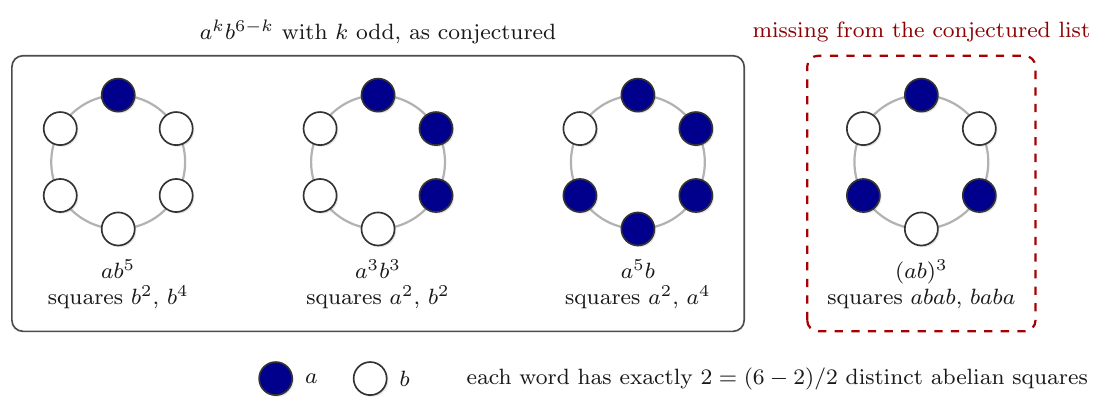
\includegraphics[width=\textwidth]{figures/fig_extremal.png}
\caption{The extremal circular words of length $6$, read clockwise from the top, up to complement. The three words on the left are those of Conjecture~0.6(b); the alternating word on the right also has exactly two distinct abelian squares.}\label{fig:extremal}
\end{figure}

Section~\ref{sec:lower} proves the lower bound by a double count of the abelian squares of half-length $m$ and $n-m$. Section~\ref{sec:tight} describes the words in which this count is tight for one letter, and Section~\ref{sec:proof} completes the proof. Section~\ref{sec:lean} describes the Lean~4 formalization.

\section{The lower bound}\label{sec:lower}

Fix a circular word $w$ of length $n\ge 1$ and set $x_i=w_{i\bmod n}$ for $i\in\Z$. For a letter $\ell$ let $t_\ell=|w|_\ell$, so $t_a+t_b=n$. For $i\in\Z$ and $L\ge 0$ let $c_\ell(i,L)$ be the number of $s\in[i,i+L)$ with $x_s=\ell$; a window of $n$ consecutive positions contains $t_\ell$ occurrences of $\ell$, so $c_\ell(i,L)<t_\ell$ implies $L<n$. For $m\ge 1$ let $W(i,m)=x_ix_{i+1}\cdots x_{i+2m-1}$; we call $W(i,m)$ a \emph{square} if $c_a(i,m)=c_a(i+m,m)$, equivalently $c_b(i,m)=c_b(i+m,m)$.

A factor of $w$ that is an abelian square has even length $2m\le n$, and it equals $W(i,m)$ for some $i$ for which $W(i,m)$ is a square. Hence
\[
D(w)=\sum_{m=1}^{\fl{n/2}}|S_m|,\qquad S_m=\{W(i,m): i\in\Z,\ W(i,m)\text{ is a square}\}.
\]

\begin{definition}\label{def:Q}
For $1\le m\le n-1$ let $Q_m$ be the set of pairs $(\ell,k)$ such that some square $W(i,m)$ satisfies $x_{i+m-1}=\ell$ and $c_\ell(i,m)=k$. For a letter $\ell$ and $k\ge 0$, the \emph{column} $C_\ell(k)$ is the set of $m\in[1,n-1]$ with $(\ell,k)\in Q_m$.
\end{definition}

So $(\ell,k)\in Q_m$ records a square of half-length $m$ whose left half ends with $\ell$ and contains $k$ letters $\ell$. The sets $S_m$, $Q_m$ and $C_\ell(k)$ do not change when $w$ is replaced by a conjugate.

\begin{lemma}\label{lem:QS}
$|Q_m|\le|S_m|$ for $1\le m\le n/2$.
\end{lemma}

\begin{proof}
The pair $(\ell,k)$ attached to a square $W(i,m)$ is determined by the word $W(i,m)$: $\ell$ is its $m$-th letter and $k$ the number of letters $\ell$ among its first $m$ letters. So $Q_m$ is the image of $S_m$ under a map.
\end{proof}

\begin{lemma}\label{lem:mirror}
Let $1\le m\le n-1$. If $(\ell,k)\in Q_m$, then $(\ell,t_\ell-k)\in Q_{n-m}$. Hence $|Q_m|=|Q_{n-m}|$, and $1\le k\le t_\ell-1$ for every $(\ell,k)\in Q_m$.
\end{lemma}

\begin{proof}
Let $W(i,m)$ be a square with $x_{i+m-1}=\ell$ and $c_\ell(i,m)=c_\ell(i+m,m)=k$. Consider $W(i+2m,n-m)$. Its left half $[i+2m,i+m+n)$ and the right half $[i+m,i+2m)$ of $W(i,m)$ together form the window $[i+m,i+m+n)$, so the left half contains $t_\ell-k$ letters $\ell$. Its right half $[i+m+n,i+2n)$ is the translate by $n$ of $[i+m,i+n)$, which together with $[i,i+m)$ forms a window of length $n$; so it also contains $t_\ell-k$ letters $\ell$. The last letter of the left half is $x_{i+m+n-1}=x_{i+m-1}=\ell$. Thus $(\ell,t_\ell-k)\in Q_{n-m}$. The map $(\ell,k)\mapsto(\ell,t_\ell-k)$ is injective and is its own inverse, so $|Q_m|=|Q_{n-m}|$. Finally $k\ge 1$ because the left half ends with $\ell$, and $t_\ell-k\ge 1$ by the same argument applied to $W(i+2m,n-m)$.
\end{proof}

\begin{figure}[ht]
\centering
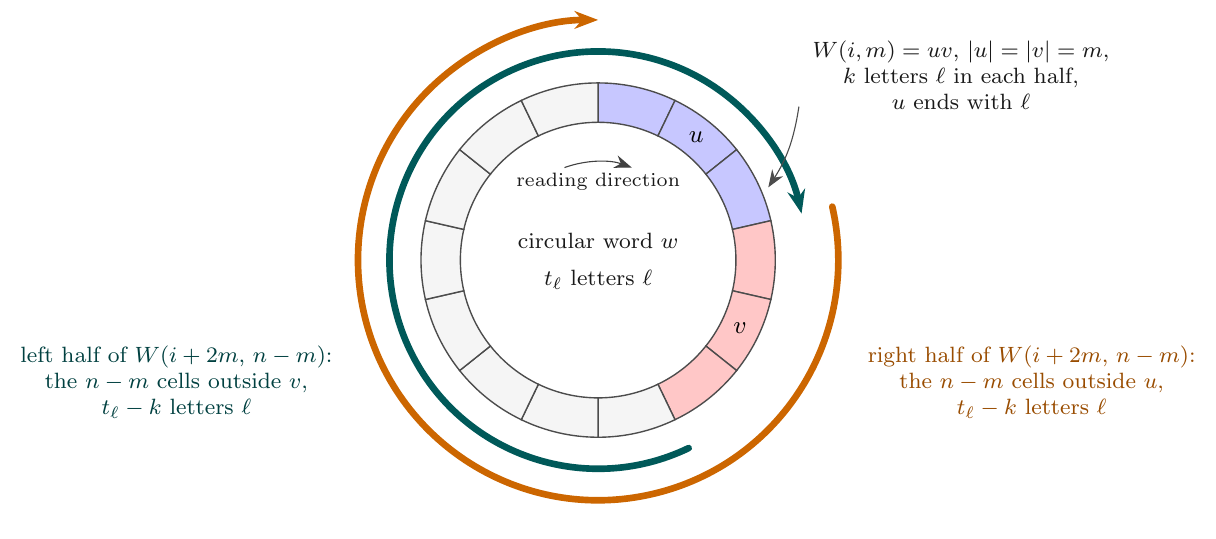
\includegraphics[width=0.92\textwidth]{figures/fig_mirror.png}
\caption{The proof of Lemma~\ref{lem:mirror}. The two halves of the square $W(i+2m,n-m)$ are the complements of $v$ and of $u$ in the circle, so each contains $t_\ell-k$ letters $\ell$, and the left one ends at the last letter of $u$.}\label{fig:mirror}
\end{figure}

If $t_\ell\ge 1$, let $(p_j)_{j\in\Z}$ be the increasing enumeration of $\{s\in\Z: x_s=\ell\}$; then $p_{j+t_\ell}=p_j+n$. For $j\in\Z$ and $1\le k<t_\ell$ let $I_j(k)$ be the interval of integers $m$ with
\begin{equation}\label{eq:interval}
\max(p_{j+k}-p_{j+1}+1,\ p_{j+2k}-p_{j+k})\ \le\ m\ \le\ \min(p_{j+k}-p_j,\ p_{j+2k+1}-p_{j+k}-1).
\end{equation}

\begin{lemma}\label{lem:interval}
Let $1\le k<t_\ell$ and $m\in I_j(k)$. Then $W(p_{j+k}+1-m,m)$ is a square whose left half ends with $\ell$ and contains $k$ letters $\ell$. In particular $m\in C_\ell(k)$.
\end{lemma}

\begin{proof}
Let $i=p_{j+k}+1-m$. By \eqref{eq:interval}, $p_j<i\le p_{j+1}$, so the left half $[i,p_{j+k}]$ contains exactly the occurrences $p_{j+1},\dots,p_{j+k}$ and ends with $x_{p_{j+k}}=\ell$. Also $p_{j+2k}\le p_{j+k}+m<p_{j+2k+1}$, so the right half $[p_{j+k}+1,p_{j+k}+m]$ contains exactly $p_{j+k+1},\dots,p_{j+2k}$. Both halves contain $k$ letters $\ell$. Since $m\ge 1$ and $k<t_\ell$, we have $1\le m<n$.
\end{proof}

\begin{figure}[ht]
\centering
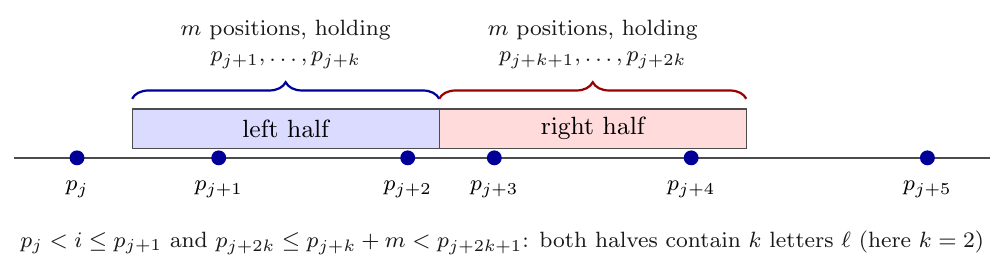
\includegraphics[width=\textwidth]{figures/fig_interval.png}
\caption{The square of Lemma~\ref{lem:interval} for $k=2$. The occurrences of $\ell$ are the dots; the left half ends at $p_{j+k}$ and the right half stops before $p_{j+2k+1}$.}\label{fig:interval}
\end{figure}

\begin{lemma}\label{lem:column}
For every letter $\ell$ and $1\le k\le t_\ell-1$, the column $C_\ell(k)$ is nonempty.
\end{lemma}

\begin{proof}
Let $d_j=p_{j+k}-p_j$ and $e_j=d_{j+k}-d_j$. Both are periodic in $j$ with period $t_\ell$, so $\sum_{j=r}^{r+t_\ell-1}e_j=0$ for every $r$. Hence some $e_{j_0}\le 0$. If $e_j\le 0$ implied $e_{j+1}<0$ for every $j$, then $e_j<0$ for all $j>j_0$, and $\sum_{j=j_0+1}^{j_0+t_\ell}e_j<0$. So there is $j$ with $e_j\le 0\le e_{j+1}$, that is $d_{j+k}\le d_j$ and $d_{j+1}\le d_{j+k+1}$. We show $I_j(k)\neq\emptyset$ by comparing each lower bound in \eqref{eq:interval} with each upper bound. First, $p_{j+k}-p_{j+1}+1\le p_{j+k}-p_j$ and $p_{j+2k}-p_{j+k}\le p_{j+2k+1}-p_{j+k}-1$. Second, $p_{j+2k}-p_{j+k}=d_{j+k}\le d_j=p_{j+k}-p_j$. Third, with $g=p_{j+k+1}-p_{j+k}\ge 1$,
\begin{align*}
p_{j+k}-p_{j+1}+1&=d_{j+1}-g+1\le d_{j+1}\le d_{j+k+1}\\
&\le d_{j+k+1}+g-1=p_{j+2k+1}-p_{j+k}-1.
\end{align*}
By Lemma~\ref{lem:interval}, $C_\ell(k)\supseteq I_j(k)\ne\emptyset$.
\end{proof}

\begin{theorem}\label{thm:lower}
$D(w)\ge\fl{(n-1)/2}$.
\end{theorem}

\begin{proof}
Let $N=\sum_{m=1}^{n-1}|Q_m|$ and $F=\sum_{m=1}^{\fl{n/2}}|Q_m|$. Counting the pairs $(m,(\ell,k))$ with $(\ell,k)\in Q_m$ by columns,
\begin{equation}\label{eq:N}
N=\sum_{\ell}\sum_{k\ge 0}|C_\ell(k)|,\qquad \sum_{k\ge 0}|C_\ell(k)|\ge t_\ell-1\ \text{ if } t_\ell\ge 1,
\end{equation}
by Lemmas~\ref{lem:mirror} and~\ref{lem:column}. If both letters occur, $N\ge t_a+t_b-2=n-2$; otherwise $N\ge n-1$. By Lemma~\ref{lem:mirror}, $|Q_m|=|Q_{n-m}|$, so
\begin{equation}\label{eq:NF}
N+\varepsilon\,|Q_{n/2}|=2F,\qquad \varepsilon=1\text{ if $n$ is even},\ \varepsilon=0\text{ if $n$ is odd}.
\end{equation}
Hence $2F\ge n-2$ and $F\ge\lceil(n-2)/2\rceil=\fl{(n-1)/2}$. By Lemma~\ref{lem:QS}, $D(w)\ge F$.
\end{proof}

We call a letter $\ell$ with $t_\ell\ge 1$ \emph{tight} if $|C_\ell(k)|\le 1$ for every $k$. By Lemmas~\ref{lem:mirror} and~\ref{lem:column}, $\ell$ is tight if and only if $\sum_k|C_\ell(k)|=t_\ell-1$. We call $w$ \emph{rigid} if $|S_m|=|Q_m|$ for $1\le m\le n/2$: two squares $W(i,m)$, $W(i',m)$ with $2m\le n$, $x_{i+m-1}=x_{i'+m-1}=\ell$ and $c_\ell(i,m)=c_\ell(i',m)$ are equal words.

\begin{proposition}\label{prop:equality}
If $D(w)=\fl{(n-1)/2}$, then $w$ is rigid and $N+\varepsilon|Q_{n/2}|=2\fl{(n-1)/2}$.
\end{proposition}

\begin{proof}
In the proof of Theorem~\ref{thm:lower}, $\fl{(n-1)/2}\le F\le D(w)$, so $F=D(w)$, and $|Q_m|\le|S_m|$ for each $m$ forces $|Q_m|=|S_m|$. Then \eqref{eq:NF} gives the second statement.
\end{proof}

\section{Rigid words with a tight letter}\label{sec:tight}

\begin{theorem}\label{thm:classify}
Let $w$ be rigid and let $\ell$ be a tight letter, $t=t_\ell$. Then $w$ is a conjugate of $\ell^t\lb^{\,n-t}$ with $t$ odd or $t=n$, or $n=2t$ and $w$ is a conjugate of $(\ell\lb)^t$.
\end{theorem}

Throughout this section $w$ and $\ell$ are as in Theorem~\ref{thm:classify}, $(p_j)$ enumerates the occurrences of $\ell$, and $g_j=p_{j+1}-p_j\ge 1$. Since $\ell$ is tight, Lemma~\ref{lem:interval} gives:
\begin{equation}\label{eq:tight}
\text{for } 1\le k<t,\ \text{the integers in } \textstyle\bigcup_j I_j(k)\ \text{form a set with at most one element.}
\end{equation}

\begin{proof}[Proof of Theorem~\ref{thm:classify}]
If $t=n$, then $w=\ell^n$. Assume $t<n$, so $g_j\ge 2$ for some $j$.

\emph{Case A: $g_j\ge 2$ for all $j$.} If $t=1$, then $w$ is a conjugate of $\ell\lb^{\,n-1}$. Let $t\ge 2$. By \eqref{eq:interval}, $I_j(1)$ is the set of $m$ with $g_{j+1}\le m\le\min(g_j,\,g_{j+1}+g_{j+2}-1)$. If $g_j>g_{j+1}$, then $I_j(1)\supseteq\{g_{j+1},g_{j+1}+1\}$ since $g_{j+2}\ge 2$, contradicting \eqref{eq:tight}. So $g_j\le g_{j+1}$ for all $j$, and as $g$ is periodic, $g_j=\delta$ is constant and $n=t\delta$. If $\delta=2$, then $n=2t$ and $w$ is a conjugate of $(\ell\lb)^t$. Let $\delta\ge 3$, so $p_{j}=p_0+j\delta$. The words $W(p_1,\delta)$ and $W(p_1+2,\delta)$ have halves $\ell\lb^{\,\delta-1}$, $\ell\lb^{\,\delta-1}$ and $\lb^{\,\delta-2}\ell\lb$, $\lb^{\,\delta-2}\ell\lb$. Both are squares whose left halves end with $\lb$ and contain $\delta-1$ letters $\lb$, and $2\delta\le n$. By rigidity they are equal, but their first letters are $\ell$ and $\lb$.

\emph{Case B: $g_j=1$ for some $j$.} A \emph{run} of length $L\ge 1$ consists of occurrences $p_{J+1},\dots,p_{J+L}$ with $g_J\ge 2$, $g_{J+1}=\dots=g_{J+L-1}=1$ and $g_{J+L}\ge 2$; its \emph{gaps} are $\lambda=g_J$ and $\rho=g_{J+L}$. Since $g$ has period $t$ and some $g_j\ge 2$, every run has length $L\le t$. The two occurrences $p_j,p_{j+1}$ with $g_j=1$ lie in a run of length at least $2$.

(B1) \emph{Every run has odd length.} Suppose a run has length $2i$, $i\ge 1$. In \eqref{eq:interval} for $I_J(i)$ the lower bounds are $i$ and $i$, and the upper bounds are $\lambda+i-1\ge i+1$ and $i+\rho-1\ge i+1$. So $I_J(i)\supseteq\{i,i+1\}$ with $i<2i\le t$, contradicting \eqref{eq:tight}.

For a run $p_{J+1},\dots,p_{J+2h+1}$ with $h\ge 1$ and gaps $\lambda,\rho$, \eqref{eq:interval} gives, with $\lambda'=g_{J-1}$ and $\rho'=g_{J+2h+2}$,
\begin{align}
I_{J-1}(h+1)&=[\lambda+h,\ \min(\lambda+h+\lambda'-1,\ h+\rho)],\label{eq:left}\\
I_J(h+1)&=[\rho+h,\ \min(\lambda+h,\ h+\rho+\rho'-1)],\label{eq:right}
\end{align}
where we used $\lambda,\rho\ge 2$. Here $h+1<2h+1\le t$.

(B2) \emph{All runs of length at least $3$ have the same length.} Let a run $p_{J+1},\dots,p_{J+2h+1}$ have $h\ge 1$, and suppose another run $p_{J'+1},\dots,p_{J'+L'}$ has $L'\ge 2h+2$. In \eqref{eq:interval} for $I_{J'}(h+1)$ the lower bounds are $h+1$ and $h+1$, and the upper bounds are at least $h+1$; so $h+1\in I_{J'}(h+1)$. By \eqref{eq:left} and \eqref{eq:right}, $\lambda+h\in I_{J-1}(h+1)$ if $\lambda\le\rho$ and $\rho+h\in I_J(h+1)$ if $\rho\le\lambda$. Both numbers exceed $h+1$, contradicting \eqref{eq:tight}.

By (B1) and (B2) there is $h\ge 1$ such that every run has length $1$ or $2h+1$, and some run has length $2h+1$. Consider such a run $R=(p_{J+1},\dots,p_{J+2h+1})$ with gaps $\lambda,\rho$.

(B3) \emph{$\rho<\lambda$ is impossible.} Let $R'$ be the run following $R$, starting at $p_{J+2h+2}$. If $R'$ has length $1$, then $\rho'\ge 2$, and by \eqref{eq:right} $I_J(h+1)\supseteq\{\rho+h,\rho+h+1\}$. If $R'$ has length $2h+1$, let $\sigma\ge 2$ be its right gap. Then $t\neq 2h+1$: otherwise $R'$ is the translate of $R$ by $n$ and $\rho=g_{J+t}=g_J=\lambda$. In \eqref{eq:interval} for $I_J(2h+1)$ the lower bounds are $2h+1$ and $2h+\rho$, and the upper bounds are $2h+\lambda\ge 2h+\rho+1$ and $2h+\rho+\sigma-1\ge 2h+\rho+1$; so $I_J(2h+1)\supseteq\{2h+\rho,2h+\rho+1\}$ with $2h+1<t$. Both cases contradict \eqref{eq:tight}.

(B4) \emph{If $\lambda<\rho$, the occurrence $p_J$ is not a run of length $1$.} Otherwise $\lambda'\ge 2$, and by \eqref{eq:left} $I_{J-1}(h+1)\supseteq\{\lambda+h,\lambda+h+1\}$, contradicting \eqref{eq:tight}.

(B5) \emph{If $\lambda=\rho$, then $t=2h+1$ and $w$ is a conjugate of $\ell^{2h+1}\lb^{\,\lambda-1}$.} By \eqref{eq:left} and \eqref{eq:right}, $m=\lambda+h$ lies in $I_{J-1}(h+1)$ and in $I_J(h+1)$. By Lemma~\ref{lem:interval} the squares $W(p_J,m)$ and $W(p_J+1,m)$ have left halves ending with $\ell$ and containing $h+1$ letters $\ell$. Their first letters are $x_{p_J}=\ell$ and $x_{p_J+1}=\lb$, since $p_J<p_J+1<p_{J+1}$. By rigidity, $2m>n$. Then $p_{J+t}=p_J+n<p_J+2\lambda+2h=p_{J+2h+2}$, so $t\le 2h+1$, and $t\ge 2h+1$ as $R$ has $2h+1$ occurrences. So $t=2h+1$, $n=p_{J+2h+2}-p_{J+1}=2h+\lambda$, and $x_{p_{J+1}}\cdots x_{p_{J+1}+n-1}=\ell^{2h+1}\lb^{\,\lambda-1}$.

Now choose the run $R$ of length $2h+1$ with the least left gap $\lambda$. By (B3), $\rho\ge\lambda$. If $\rho=\lambda$, (B5) applies. If $\rho>\lambda$, then by (B4) the run $R^-$ preceding $R$ has length $2h+1$. Its right gap is $\lambda$, and its left gap is at least $\lambda$ by the choice of $R$; by (B3) the two are equal, and (B5) applies to $R^-$. In all cases $w$ is a conjugate of $\ell^{t}\lb^{\,n-t}$ with $t=2h+1$ odd.
\end{proof}

\section{Proof of Theorem~\ref{thm:main}}\label{sec:proof}

\begin{lemma}\label{lem:upper}
Let $\ell$ be a letter.
\begin{enumerate}
\item[(i)] Let $0\le\alpha\le n$ and $\beta=n-\alpha$, and suppose each of $\alpha$, $\beta$ is $0$, odd, or at least $n-1$. Then every abelian square factor of the circular word $\ell^\alpha\lb^{\,\beta}$ is $\ell^{2m}$ or $\lb^{\,2m}$, and $D(\ell^\alpha\lb^{\,\beta})=\fl{\alpha/2}+\fl{\beta/2}$.
\item[(ii)] For even $n$, $D((\ell\lb)^{n/2})=2\fl{n/4}$.
\end{enumerate}
\end{lemma}

\begin{proof}
(i) Let $s=uv$ be an abelian square factor, $|u|=|v|=m$, $2m\le n$, containing both letters; then $1\le\alpha,\beta\le n-1$, and read cyclically the word consists of the two blocks $\ell^\alpha$ and $\lb^{\,\beta}$. If $s$ crosses exactly one block boundary, $s=c^r\bar c^{\,2m-r}$ with $c\in\{\ell,\lb\}$ and $0<r<2m$, and $|u|_c=\min(r,m)>\max(r-m,0)=|v|_c$. Otherwise $s$ contains a whole block in its interior, say $s=\ell^r\lb^{\,\beta}\ell^{r'}$ with $r,r'\ge 1$. Then $\beta\le 2m-2\le n-2$, so $\beta$ is odd, whereas $\beta=|s|_{\lb}=2|u|_{\lb}$. The case $s=\lb^{\,r}\ell^\alpha\lb^{\,r'}$ is symmetric. The factor $\ell^{2m}$ occurs if and only if $2m\le\alpha$, and $\lb^{\,2m}$ if and only if $2m\le\beta$.

(ii) Every factor of length $2m$ alternates. If $m$ is odd, its halves start with different letters $c\ne\bar c$, and $|u|_c=(m+1)/2\ne(m-1)/2=|v|_c$. If $m$ is even, both halves contain $m/2$ letters of each kind, and there are exactly two factors of length $2m\le n$. So $D=2\,|\{m: m\text{ even},\ 2\le m\le n/2\}|=2\fl{n/4}$.
\end{proof}

\begin{lemma}\label{lem:fat}
Let $\alpha\ge 3$, $h\ge 1$, $n=\alpha+2h$ and $w=\ell^\alpha\lb^{\,2h}$. Then $C_{\lb}(h)\supseteq\{h,\,h+1,\,n-h\}$, three distinct numbers.
\end{lemma}

\begin{proof}
$W(\alpha,h)=\lb^{\,2h}$ is a square whose left half $\lb^{\,h}$ ends with $\lb$, so $h\in C_{\lb}(h)$. $W(\alpha-1,h+1)=\ell\lb^{\,2h}\ell$ is a square with halves $\ell\lb^{\,h}$ and $\lb^{\,h}\ell$, and $2h+2\le n$; so $h+1\in C_{\lb}(h)$. By Lemma~\ref{lem:mirror} with $t_{\lb}=2h$, $n-h\in C_{\lb}(2h-h)$. Finally $n-h=\alpha+h\ge h+3$.
\end{proof}

\begin{proof}[Proof of Theorem~\ref{thm:main}]
The lower bound is Theorem~\ref{thm:lower}. If $w$ is a conjugate of a word in the list, Lemma~\ref{lem:upper} gives $D(w)=\fl{(n-1)/2}$: for $a^n$ ($n$ odd) $\fl{n/2}=(n-1)/2$; for $a^{n-1}b$ ($n$ odd) $(n-1)/2+0$; for $a^kb^{n-k}$ ($n$ even, $k$ odd) $(k-1)/2+(n-k-1)/2=(n-2)/2$; for $(ab)^{n/2}$ ($n\equiv 2\pmod 4$) $2(n-2)/4$. Complements and conjugates have the same $D$.

Conversely let $D(w)=\fl{(n-1)/2}$. By Proposition~\ref{prop:equality}, $w$ is rigid and $N+\varepsilon|Q_{n/2}|=2\fl{(n-1)/2}$.

\emph{$n$ even.} Then $N+|Q_{n/2}|=n-2$. If only one letter occurs, $N\ge n-1$; so both occur, and by \eqref{eq:N} $N\ge n-2$. Hence $|Q_{n/2}|=0$ and $\sum_k|C_\ell(k)|=t_\ell-1$ for both letters, so both letters are tight. Theorem~\ref{thm:classify} for $\ell=a$ shows that $w$ is a conjugate of $a^kb^{n-k}$ with $k$ odd ($k=n$ is excluded since $b$ occurs), or $n=2t_a$ and $w$ is a conjugate of $(ab)^{n/2}$. In the second case, if $n\equiv 0\pmod 4$, both halves of $W(0,n/2)$ alternate and have even length $n/2$, so $W(0,n/2)$ is a square and $Q_{n/2}\ne\emptyset$, a contradiction. So $n\equiv 2\pmod 4$.

\emph{$n$ odd.} Then $N=n-1$. If only one letter occurs, $w$ is $a^n$ or $b^n$. Otherwise \eqref{eq:N} gives $\sum_k|C_a(k)|+\sum_k|C_b(k)|=(t_a-1)+(t_b-1)+1$ with $\sum_k|C_\ell(k)|\ge t_\ell-1$ for both letters. So one letter $\ell$ is tight, and $\sum_k|C_{\lb}(k)|\le t_{\lb}$. By Theorem~\ref{thm:classify}, $w$ is a conjugate of $\ell^t\lb^{\,n-t}$ with $t=t_\ell$ odd, since $t<n$ and $n$ is odd. Then $n-t=2h$ with $h\ge 1$. If $t=1$, then $w$ is a conjugate of $\lb^{\,n-1}\ell$. If $t\ge 3$, Lemma~\ref{lem:fat} gives $|C_{\lb}(h)|\ge 3$ with $1\le h<2h=t_{\lb}$, and with Lemma~\ref{lem:column}, $\sum_k|C_{\lb}(k)|\ge(t_{\lb}-1)+2>t_{\lb}$, a contradiction.
\end{proof}

\section{Formal verification}\label{sec:lean}

Theorem~\ref{thm:main} and Corollary~\ref{cor:simpson} are formalized in Lean~4 \cite{MU21} with Mathlib \cite{Mathlib20}, version~4.34.1, and the formal proofs are checked by the Lean kernel. Words are lists over a two-letter alphabet, and the definitions follow Section~\ref{sec:intro} literally: an abelian square is a word $uv$ with $u$ nonempty and the same number of each letter in $u$ and $v$; the factors of a circular word $w$ of length $n$ are the prefixes of length $L$, $1\le L\le n$, of its $n$ rotations; and $D(w)$ is the number of distinct factors that are abelian squares. The formal statements are the following. For every $n\ge 1$ the least value of $D$ on the words of length $n$ is $\fl{(n-1)/2}$. A word of odd length, and a word of even length, attains this value exactly when it is a conjugate of one of the words in (a), respectively (b), of Theorem~\ref{thm:main}. Part~(a) of Conjecture~0.6 holds, and part~(b), stated literally, is false. Finally $D(ababab)=2$, and $ababab$ is not a conjugate of $a^kb^{6-k}$ or of its complement for any $k$. The repository verification of the pinned source checks these statements; the verification record accompanying this edition identifies the commit and successful run. The proofs depend only on the axioms of Lean's logic, namely propositional extensionality, choice and the soundness of quotients; they contain no unproved step and add no axiom.

Independent computations confirm Theorem~\ref{thm:main} on every binary circular word of length at most $22$ and on one word of each necklace class up to length $28$, and they confirm each lemma of Sections~\ref{sec:lower} and~\ref{sec:tight} on every word of length at most $16$.

\section*{Declaration of generative AI and AI-assisted technologies in the manuscript preparation process}
Claude (Anthropic) assisted with the original proofs, Lean formalization, computations and manuscript preparation. OpenAI Codex assisted with the source audit, small-case verification and conversion to the amsart format for this edition. The mathematical proof body is retained. The author is responsible for the content; no AI system is an author.

\section*{Data availability}
\begingroup\raggedright
Deep Bhattacharjee computed the Lean formalization and the Julia, C, C++, shell and Python computations with the help of AI assistance (Claude, Anthropic). The Lean formalization of the proofs in this paper and the programs are in release~v2.2.0 of the repository \url{https://github.com/creelie/literate-octo-lamp}, \url{\releaseURL}; the earlier preprint is Hexagon \href{https://hexagonmath.org/2610.00473v1}{2610.00473v1}.\par
\endgroup

\section*{Competing interests}
None.

\section*{Funding}
None.

\begin{thebibliography}{8}

\bibitem{Sim18}
J.~Simpson, Solved and unsolved problems about abelian squares, preprint (2018), \href{https://arxiv.org/abs/1802.04481v1}{arXiv:1802.04481v1}.

\bibitem{FSP97}
A.\,S.~Fraenkel, J.~Simpson, M.~Paterson, On weak circular squares in binary words, in: Combinatorial Pattern Matching (CPM 1997), Lecture Notes in Computer Science, Springer, 1997, pp.~76--82, \href{https://doi.org/10.1007/3-540-63220-4_51}{doi:10.1007/3-540-63220-4\_51}.

\bibitem{FMMS26}
S.\,Z.~Fazekas, A.~Mammoliti, R.~Merca\c{s}, J.~Simpson, Binary words containing few abelian squares, preprint (2026), \href{https://arxiv.org/abs/2604.23188v1}{arXiv:2604.23188v1}.

\bibitem{FM15}
G.~Fici, F.~Mignosi, Words with the maximum number of abelian squares, in: Combinatorics on Words (WORDS 2015), Lecture Notes in Computer Science, Springer, 2015, pp.~122--134, \href{https://doi.org/10.1007/978-3-319-23660-5_11}{doi:10.1007/978-3-319-23660-5\_11}.

\bibitem{FMS17}
G.~Fici, F.~Mignosi, J.~Shallit, Abelian-square-rich words, Theoret. Comput. Sci. 684 (2017) 29--42, \href{https://doi.org/10.1016/j.tcs.2017.02.012}{doi:10.1016/j.tcs.2017.02.012}.

\bibitem{FP23}
G.~Fici, S.~Puzynina, Abelian combinatorics on words: a survey, Comput. Sci. Rev. 47 (2023) 100532, \href{https://doi.org/10.1016/j.cosrev.2022.100532}{doi:10.1016/j.cosrev.2022.100532}.

\bibitem{MU21}
L.~de~Moura, S.~Ullrich, The Lean~4 theorem prover and programming language, in: Automated Deduction -- CADE 28, Lecture Notes in Computer Science, Springer, 2021, pp.~625--635, \href{https://doi.org/10.1007/978-3-030-79876-5_37}{doi:10.1007/978-3-030-79876-5\_37}.

\bibitem{Mathlib20}
The mathlib Community, The Lean mathematical library, in: Proceedings of the 9th ACM SIGPLAN International Conference on Certified Programs and Proofs (CPP 2020), ACM, 2020, pp.~367--381, \href{https://doi.org/10.1145/3372885.3373824}{doi:10.1145/3372885.3373824}.

\end{thebibliography}

\end{document}
